\chapter{Analysis of the Diffusion of Power in the Tor Network in Three Dimensions}

\setcounter{footnote}{145} % Continue numbering from Chapter 3

The third chapter of this dissertation aims to present the analyses of diffusion of power in three dimensions carried out from a database composed of information derived from journalistic articles. The database presents the variables ``authority,'' ``control,'' and ``outcomes'' that emerge from the operationalization of the three dimensions of the same name. In order to provide context for the variables, we also identified other relevant information such as the identification of peers and stakeholders (relative to the authority dimension), the object considered relevant for achieving the desired outcome by the non-state actor in the context of the article (relative to the control dimension), and the effect on reality (relative to the ``outcomes'' dimension). In addition, the database is composed of other information related to the identification of the newspaper articles such as authors, newspapers, country of headquarters, article title, etc.

The analysis was conducted according to the methodology defined in the Introduction of this dissertation and uses the operationalization of the phenomenon of diffusion of power -- based on the frequency of occurrences of each variable, which allowed us to generate statistical tables. For the purposes of this dissertation, from the readings of the articles we identified non-state actors and grouped them according to themes common to them. From this, we will present the results of the diffusion of power analysis in three dimensions -- authority, control, and outcomes: for each dimension, the results of (a) the individual analysis of each thematic group, (b) the comparative analysis between thematic groups, and (c) the general analysis of total occurrences were presented. The charts, tables, and figures that emerged from the interpretation of the data, together with the database of 139 occurrences, can be found in the appendix of this dissertation.

\section{Journalistic Frequency Regarding the Tor Network}

In order to understand the publicity given by these newspapers to the topic of the anonymous network, we examined the number of articles published per year and, thus, obtained the following chart.

% CHART 1 - NUMBER OF ARTICLES RELATED TO "Tor NETWORK" PUBLISHED PER YEAR (2007-2017)
\begin{figure}[H]
\centering
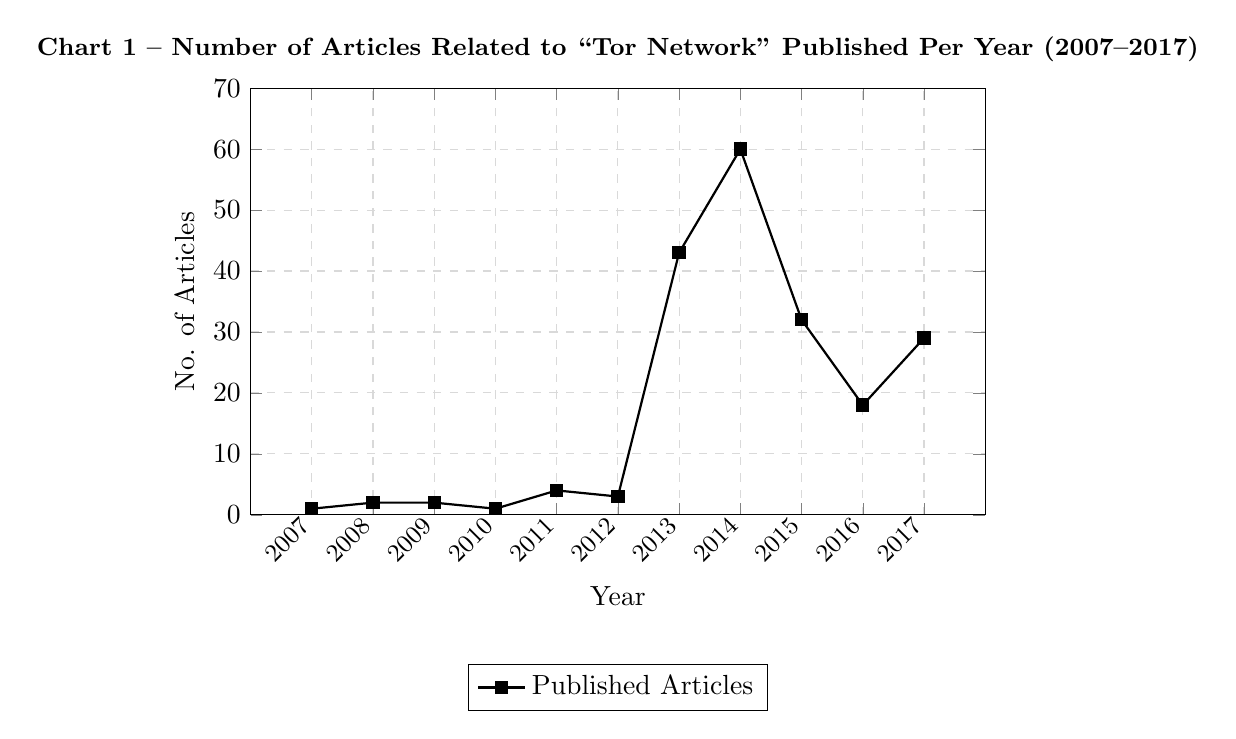
\begin{tikzpicture}
\begin{axis}[
    title={\textbf{Chart 1 -- Number of Articles Related to ``Tor Network'' Published Per Year (2007--2017)}},
    title style={align=center, font=\small\bfseries},
    xlabel={Year},
    ylabel={No. of Articles},
    ymin=0, ymax=70,
    xtick={2007,2008,2009,2010,2011,2012,2013,2014,2015,2016,2017},
    xticklabel style={rotate=45, anchor=east, font=\small},
    xticklabel={\pgfmathprintnumber[fixed, precision=0, 1000 sep={}]\tick},
    ytick={0,10,20,30,40,50,60,70},
    width=0.9\textwidth,
    height=7cm,
    grid=major,
    grid style={dashed, gray!30},
    legend style={at={(0.5,-0.35)}, anchor=north},
]
\addplot[color=black, mark=square*, thick] coordinates {
    (2007,1) (2008,2) (2009,2) (2010,1) (2011,4) (2012,3)
    (2013,43) (2014,60) (2015,32) (2016,18) (2017,29)
};
\legend{Published Articles}
\end{axis}
\end{tikzpicture}
\caption*{Source: Author.}
\end{figure}

The 195 articles were distributed over a period of one decade, as shown above. From this chart, we can make some observations regarding the average number of articles published prior to 2013, the growth in the number of publications in 2013--2014 and 2017, and the change in level after 2014.

Initially, between the years 2007 and 2012, we observed few articles published by the aforementioned newspapers -- 13 articles in total. This average changes in the following years. In 2013, the number of published articles surpassed the mark of 40. Three subjects were mainly responsible for this increase: (1) the activist organization Tor Project, responsible for the maintenance, improvement, and operationalization of the anonymous network, was cited throughout the news stories that highlighted the Tor network itself or the topic of the Dark Web; (2) the anonymous online marketplace Silk Road, whose main administrator, Ross Ulbricht, was imprisoned by North American authorities in October 2013; (3) and the revelations of Edward Snowden, which exposed the global surveillance scheme perpetrated by the US government and its allies.\footnote{See ``Appendix 5 -- Articles Published in 2013.''}

In 2014, the number of publications reached the level of 60 articles -- 50\% more than the previous year. In addition to the subjects mentioned earlier, three others also contributed to the increase: (a) the rise of the online marketplace Silk Road 2.0, which sought to continue the previous version closed in 2013 by US law enforcement authorities; (b) the operation of transnational child pornography networks through the anonymous network; (c) and the exposure of the topic of privacy and anonymity on the Internet.\footnote{See ``Appendix 6 -- Articles Published in 2014.''}

While in the period of 2013 and 2014 there was growth in the number of published articles related to the Tor anonymous network, in the following years a decrease in the number of these publications occurred. Only in 2017 was there a slight increase. It is relevant to note that after 2014, publications related to the Tor anonymous network shifted to a higher level compared to the period before 2013: previously they did not reach 10 publications per year, and afterward they published no fewer than 15 news articles. This change in level reflects the interest of journalistic coverage in, primarily, the so-called ``anonymous markets'' of the Dark Web. These markets are known especially for trading drugs, narcotics, and other illicit substances. In 2017, for example, the Alphabay marketplace dominated journalistic publications involving the Tor anonymous network. But the change in level also reflects the journalistic coverage given to the arrests of administrators and those responsible for child pornography networks by police authorities of various governments.\footnote{See ``Appendix 7 -- Articles Published in 2017.''}

During this ten-year period, the British newspapers The Guardian and Mail Online and the American newspaper The Washington Post were those that produced the most news articles related to the Tor anonymous network. The Eastern newspapers, Tribune Newspaper, People's Daily Online, and Xinhua News Agency, were those that gave the least publicity to the topic.

% TABLE 4 - NUMBER OF ARTICLES RELATED TO "Tor NETWORK" PUBLISHED BY EACH NEWSPAPER (2007-2017)
\begin{table}[H]
\centering
\caption{Number of Articles Related to ``Tor Network'' Published by Each Newspaper (2007--2017)}
\begin{tabular}{llc}
\toprule
\textbf{Country} & \textbf{Newspaper} & \textbf{N} \\
\midrule
England & The Guardian & 64 \\
England & Mail Online* & 53 \\
USA & Washington Post & 31 \\
England & Telegraph Media Group & 17 \\
USA & Advance Digital** & 17 \\
USA & The NY Times & 11 \\
India & Tribune Newspapers & 1 \\
China & People's Daily Online & 1 \\
USA & Hearst Newspapers & 0 \\
China & Xinhua News Agency & -- \\
\midrule
 & \textbf{Total} & \textbf{195} \\
\bottomrule
\end{tabular}
\end{table}

